\subsection*{Træning og evaluering}
Træningen er opdelt i tre boundarys, hvor de to er aktive under træningen samt ved stop træning. Den sidste boundary er aktiv efter træningen, idet træningen skal evalueres. Der er til disse tre boundarys opstillet en fælles controller. Boundarys og controller fremgår af \autoref{fig:DesignTraening}. 

\begin{figure} [H]
\centering
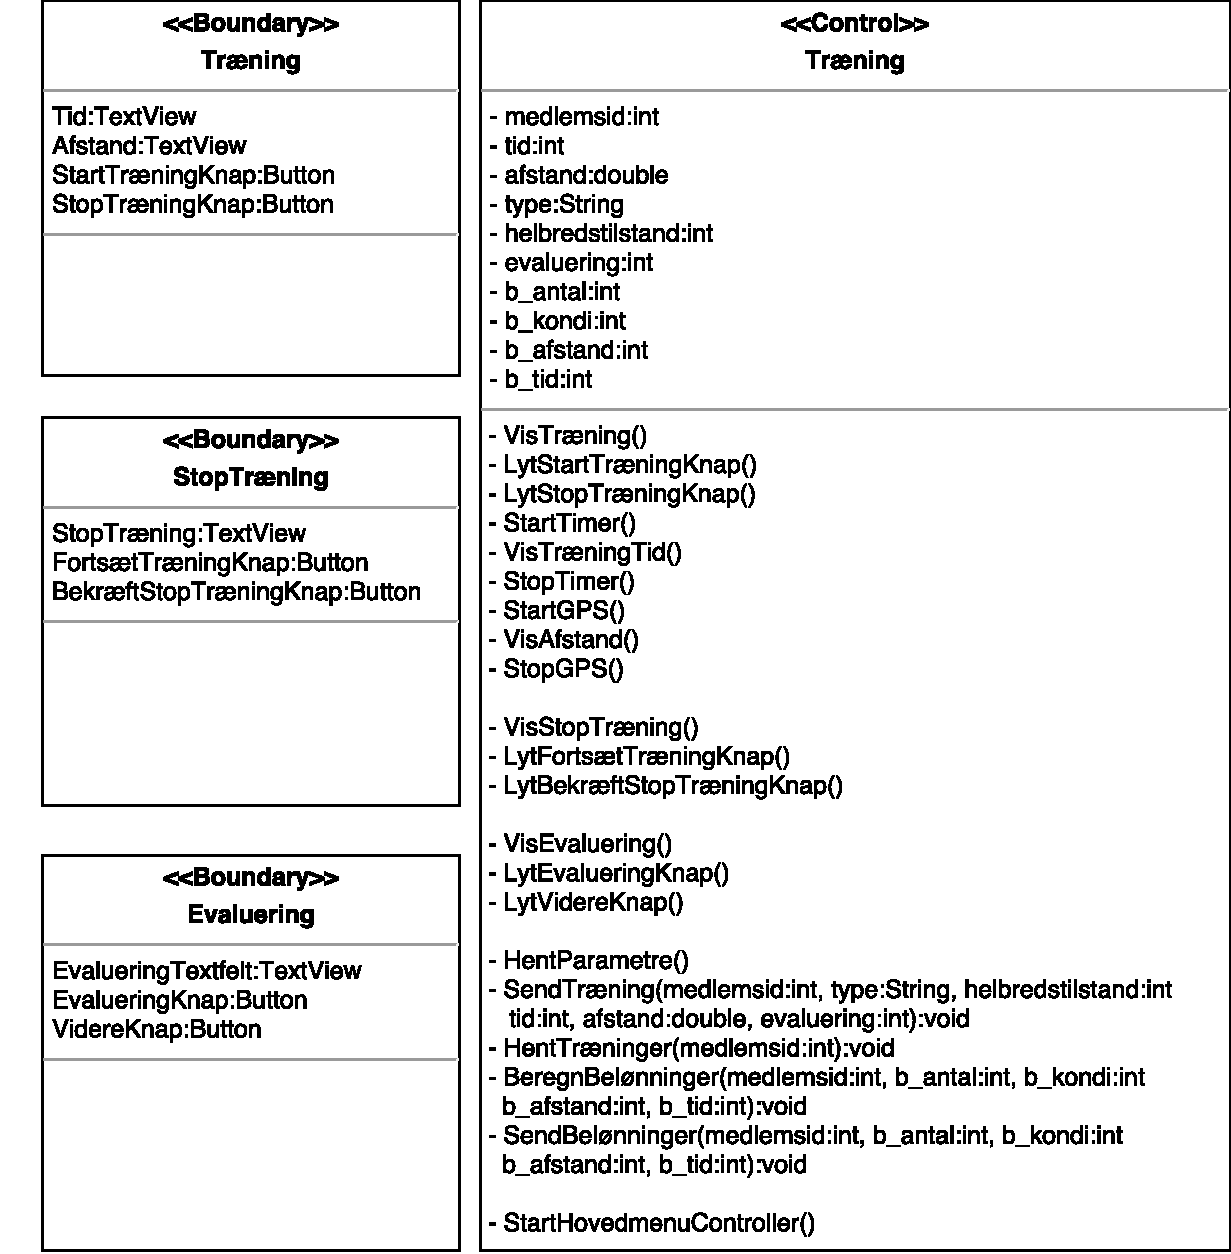
\includegraphics[width=0.7\textwidth]{figures/MVC/MVCTraening}
\caption{Designklasser for træning samt evaluering. Til venstre fremgår boundarys for Træning, StopTræning og Evaluering. Den tilhørende controller ses til højre.}
\label{fig:DesignTraening}
\end{figure}

\noindent
Grænsefladen for \textit{Træning}, \textit{StopTræning} og \textit{Evaluering} indeholder tekstfelter og knapper af typen TextView og Button. Controlleren \textit{TræningEvaluering} indeholder metoderne Lyt, Vis, Start, Hent, Stop og Send. 

I sammenspil med designklasserne er der udarbejdet et sekvensdiagram, hvilket fremgår af \autoref{fig:SEKTraening}. 

\begin{figure} [H]
\centering
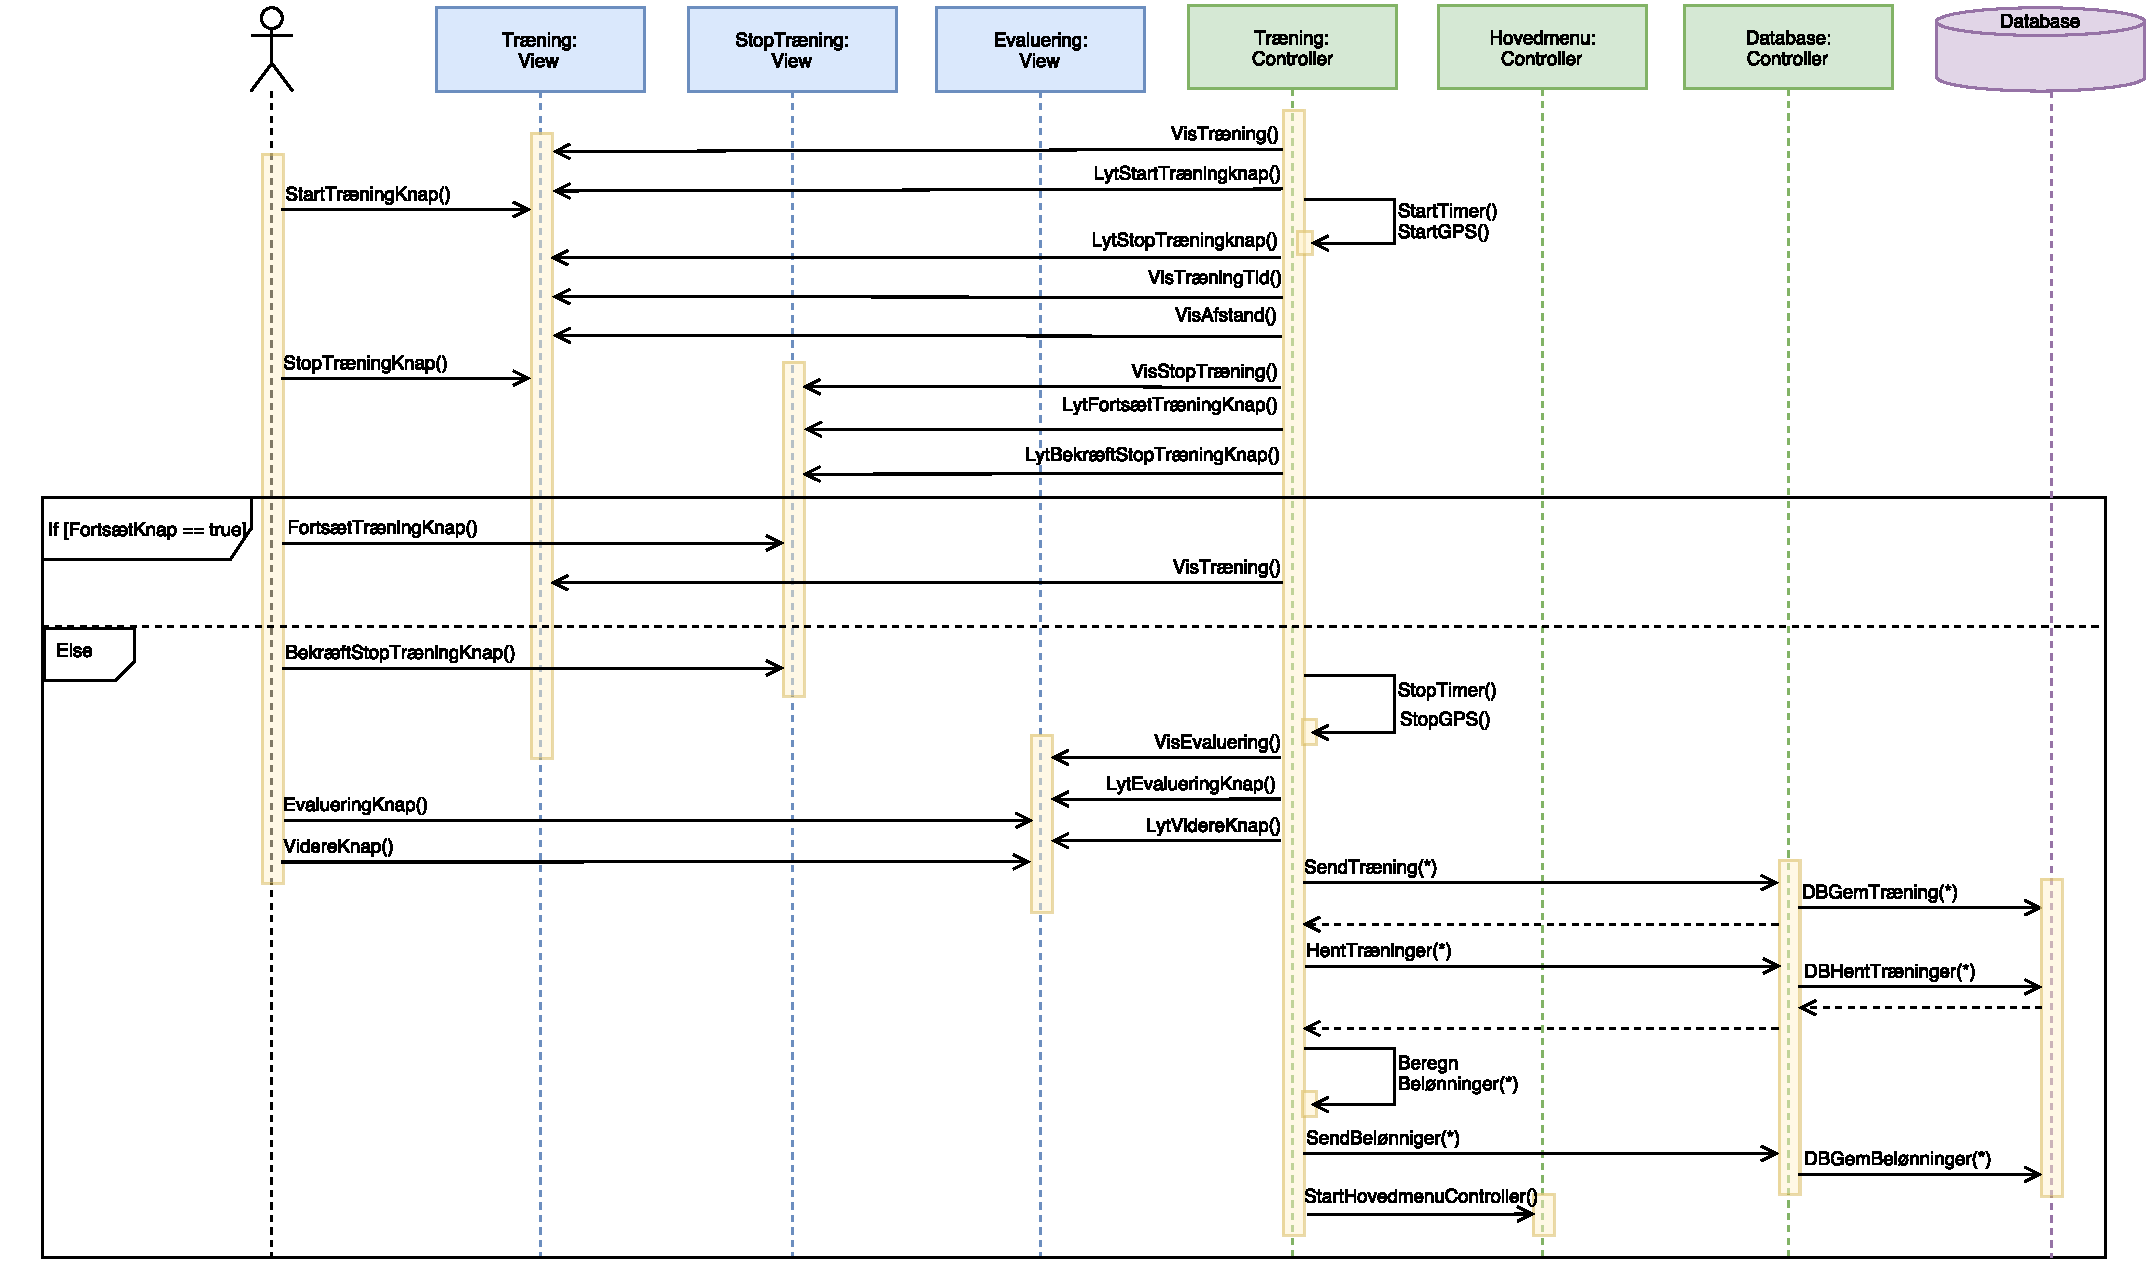
\includegraphics[width=1.55\textwidth, angle=90]{figures/Sek/SEKTraening}
\caption{Sekvensdiagram for træning. \fxnote{Hvor skal ting gemmes?}}
\label{fig:SEKTraening}
\end{figure}

\noindent
\textit{Træning} er den første grænseflade, der vises ved en igangværende træning. Controlleren \textit{TræningEvaluering} starter timer og GPS. Herefter vises tiden og afstanden i grænsefladen. Controlleren henter målinger fra kompatible enheder, hvis disse er tilsluttet og viser dem. \fxnote{OBS!! Dette er stadig lidt uklart}. Brugeren kan under træningen, eller når træningen er fuldført, afslutte ved at trykke på StopTræningKnap, hvorefter grænsefladen for \textit{StopTræning} vises. I denne grænseflade har brugeren mulighed for at trykke på FortsætTræningKnap eller BekræftStopTræningKnap. Vælges FortsætTræningKnap vises grænsefladen for \textit{Træning} igen og brugeren kan fortsætte træningen. Vælges BekræftStopTræningKnap stopper controlleren med at lagre data fra GPS, timer og eventuelle kompatible måleenheder. Herefter vises grænsefladen \textit{Evaluering}, hvor brugeren skal angive en evaluering af dagens træning. Evaluering bekræftes ved VidereKnap. Herefter sender controlleren træningsoplysninger til controlleren for \textit{Database}, som gemmer træningen i \textit{Database} \fxnote{Hvad gør vi i forhold til dette?}. Herefter gives der besked til \textit{Hovedmenu} controlleren om at vise hovedmenuen.




%Denne indeholder tekstfelter, hvori tiden samt afstanden oplyses. Derudover er der et tekstfelt til kompatiblemålinger, hvis disse er tilsluttet. Da \textit{TræningsGrænsefladen} skal oplyse målinger fra tilkoblede kompatible måleenheder, skal denne grænseflade ligeledes styres af \textit{TilkoblingafkompatibleenhederController}, der ses af \autoref{fig:kompatiblemåleenheder}. Yderligere indeholder denne grænseflade en stopknap, af typen button, hvis træningen ønskes afsluttet. 
%Ønskes træningen afsluttet vises \textit{StopTræningGrænseflade}, hvori der er opstillet et tekstfelt samt to knapper. Tekstfeltet informerer brugeren om, at vedkommende er ved at afslutte træningen, hvorved brugeren kan bekræfte, at træningen skal stoppes eller fortsætte træningen ved hjælp af de opstillede knapper. 
%Efter en afsluttet træning, skal træningen evalueres, hvilket forekommer i \textit{EvalueringGrænsefladen}. Denne grænseflade indeholder et tekstfelt, der informerer brugeren om evalueringen, samt fire knapper. De tre knapper er opstillet således brugeren kan evaluere den udførte træning. Evalueringen bekræftes ved, at benytte den sidste knap til at bevæge sig videre i app’en. 
%\textit{TræningEvalueringController} er den fælles controller, som bestemmer, hvilken boundary, som vises. Denne controller lagrer tiden, afstanden, evaluering samt kompatible målinger, hvis disse er tilkoblet. Derudover lytter controlleren på de forskellige respektive knapper og håndterer skiftet mellem boundarys. Idet brugeren har evalueret sin træning og bekræftet ved at benytte videreknappen sendes alle træningsoplysningerne til databasen, hvori de gemmes. Dertil returneres brugeren til hovedmenuen. 
